\documentclass[sigplan,10pt]{acmart}\settopmatter{printfolios=true,printccs=false,printacmref=false}

\usepackage{lineno,hyperref,xcolor}
\usepackage{stmaryrd}
\usepackage{amssymb}
\usepackage{xypic}
\usepackage{semantic}
\usepackage{booktabs} 
\usepackage{subcaption}

\acmConference[PL'17]{ACM SIGPLAN Conference on Programming Languages}{January 01--03, 2017}{New York, NY, USA}
\acmYear{2017}
\acmISBN{} % \acmISBN{978-x-xxxx-xxxx-x/YY/MM}
\acmDOI{} % \acmDOI{10.1145/nnnnnnn.nnnnnnn}
\startPage{1}
\setcopyright{none}
\bibliographystyle{ACM-Reference-Format}

\title{Design and implementaiton of a live coding environment}

\author{Tomas Petricek}
\affiliation{
  \institution{The Alan Turing Institute}
  \country{London, United Kingdom}
}
\email{tomas@tomasp.net}


\definecolor{cmtclr}{rgb}{0.0,0.6,0.0}
\definecolor{kvdclr}{rgb}{0.0,0.0,0.6}
\definecolor{numclr}{rgb}{0.0,0.4,0.0}
\definecolor{strclr}{rgb}{0.4,0.3,0.0}
\definecolor{prepclr}{rgb}{0.6,0.0,0.2}
\newcommand{\vect}[1]{\langl #1 \rangl}
\newcommand{\langl}{\begin{picture}(4.5,7)
\put(1.1,2.5){\rotatebox{60}{\line(1,0){5.5}}}
\put(1.1,2.5){\rotatebox{300}{\line(1,0){5.5}}}
\end{picture}}
\newcommand{\rangl}{\begin{picture}(4.5,7)
\put(.9,2.5){\rotatebox{120}{\line(1,0){5.5}}}
\put(.9,2.5){\rotatebox{240}{\line(1,0){5.5}}}
\end{picture}}
\newcommand{\ball}[1]{\FPeval{\result}{clip(201+#1)}\textnormal{\ding{\result}}}
\newcommand{\lsep}{~\,|\,~}
\newcommand{\num}[1]{\textcolor{numclr}{#1}}
\newcommand{\str}[1]{\textnormal{\textcolor{strclr}{\sffamily "#1"}}}
\newcommand{\ident}[1]{\textnormal{\sffamily #1}}
\newcommand{\qident}[1]{\textnormal{\sffamily \guillemotleft #1\guillemotright}}
\newcommand{\dom}{\ident{dom}}
\newcommand{\kvd}[1]{\textnormal{\textcolor{kvdclr}{\sffamily #1}}}

\newcommand{\bndclr}[1]{\textcolor{kvdclr}{#1}}
\newcommand{\bkndclr}[1]{\textcolor{prepclr}{#1}}
\newcommand{\blblclr}[1]{\textcolor{numclr}{#1}}
\newcommand{\bnd}[1]{\textnormal{\textcolor{kvdclr}{\sffamily #1}}}
\newcommand{\bknd}[1]{\textnormal{\textcolor{prepclr}{\sffamily #1}}}
\newcommand{\blbl}[1]{\textnormal{\textcolor{numclr}{\sffamily #1}}}


\begin{document}
\begin{abstract}
Lorem ipsum dolor sit amet, consectetur adipisicing elit, sed do eiusmod tempor incididunt ut labore et dolore magna aliqua. Ut enim ad minim veniam, quis nostrud exercitation ullamco laboris nisi ut aliquip ex ea commodo consequat. Duis aute irure dolor in reprehenderit in voluptate velit esse cillum dolore eu fugiat nulla pariatur. Excepteur sint occaecat cupidatat non proident, sunt in culpa qui officia deserunt mollit anim id est laborum.

Ut enim ad minim veniam, quis nostrud exercitation ullamco laboris nisi ut aliquip ex ea commodo consequat. Duis aute irure dolor in reprehenderit in voluptate velit esse cillum dolore eu fugiat nulla pariatur. Excepteur sint occaecat cupidatat non proident, sunt in culpa qui officia deserunt mollit anim id est laborum.
\end{abstract}
\maketitle

% ==================================================================================================

\section{Introduction}
One of the aspects that make spreadsheet tools such as Excel more accessible than programming 
environments is their liveness. When you change a value in a cell in Excel, the whole spreadsheet
is updated instantly and you see the new results immediately.

Increasing number of programming environments aim to provide the same live experience for more
standard programming languages, but doing this is not easy. Fully recomputing the whole program after
every single change is inefficient and calculating how a change in source code changes the result
is extremely hard when the editor allows arbitrary manipulation of program text. For example, 
consider the following simple program that gets the release years of 10 most expensive movies 
in a data set \ident{movies}:
%
\begin{equation*}
\begin{array}{l}  
\kvd{let}~\ident{top} =\ident{movies}\\
\quad .\ident{sortBy}(\lambda x \rightarrow x.\ident{getBudget}())\ident{.take}(\num{10})\\
\quad .\ident{map}(\lambda x \rightarrow x.\ident{getReleased()}.\ident{format}(\str{yyyy}))}\\
\end{array}
\end{equation*}
%
A live coding environment shows a preview of the list of dates \ident{top} and the programmer then
changes the code by making $\num{10}$ a variable and changing the date format to see the full date:

\begin{equation*}
\begin{array}{l}  
\kvd{let}~\ident{count} = \num{10}\\
\kvd{let}~\ident{top} = \ident{movies}\\
\quad .\ident{sortBy}(\lambda x \rightarrow x.\ident{getBudget}())\ident{.take}(\ident{count})\\
\quad \ident{.map}(\lambda x \rightarrow x.\ident{getReleased()}.\ident{format}(\str{dd-mm-yyyy}))}\\
\end{array}
\end{equation*}
%
Ideally, the live coding environment should understand the change, reuse a cached result of the
first two transformations (sorting and taking 10 elements) and only evaluate the last \ident{map}
and format the release dates of already computed top 10 movies.

This is not difficult to achieve if we represent the program in a structured way and allow the user
to edit code only via well-understood primitive operations such as ``extract variable'' (which has
no effect on the result) or ``change constant value'' (which forces recomputation of subsequent
transformations). However, many programmers still prefer to edit programs as free form text.
In this paper, we present the design and implementation of a live coding system that is capable
of reusing previously evaluated expressions as in the example above, yet, is integrated into an
ordinary text editor.

The motivation for this paper is twofold. First, implementing a live programming system requires
a different way of thinking about compilers and interpreters than the one presented in classic
programming language literature. Second, an increasing number of programming environments 
incorporate aspects of live programming [X,Y], yet relatively little has been written on their
architecture and implementation.

% --------------------------------------------------------------------------------------------------

\begin{figure*}
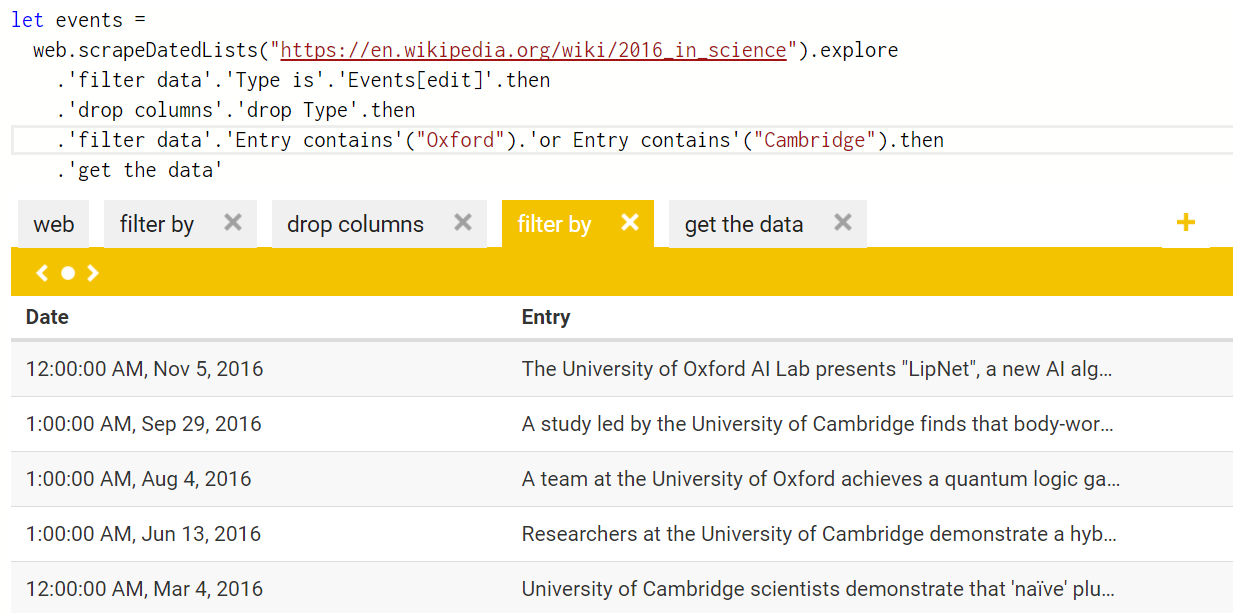
\includegraphics[scale=0.45]{scrape.png}
\caption{xxx}  
\end{figure*}

\newpage

% ==================================================================================================

\section{Live programming for data exploration}

The Gamma introduction and what this tries to do. See pretty screenshot.

This is what we care about - it's not live programming for your typical haskell,
but for R or Python.

\newpage

% ==================================================================================================

\section{Formalising live coding environment}

In this section, we present a formalisation of a live coding environment for a small,
expression-based programming language that supports \kvd{let} binding, member invocations
and $\lambda$ abstractions. This is the necessary minimum for data exploration as described
in the previous section and it excludes constructs such as a mechanism for defining new objects.
%
\begin{equation*}
\begin{array}{lcl}
e &=& \kvd{let}~x = e~\kvd{in}~e ~|~ \lambda x\rightarrow e ~|~ e.m(e, \ldots, e) ~|~ x ~|~ n
\end{array}
\end{equation*}
%
Here, $m$ ranges over member names, $x$ over variables and $n$ over primitive values such as 
numbers. Function values can be passed as arguments to methods (provided by a type provider), but 
for the purpose of this paper, we do not need to be able to invoke them directly.

\paragraph{The problem with functions.}
In the context of live programming, \kvd{let} binding and member access are unproblematic.
We can evaluate them and provide live preview for both of them, including all their sub-expressions.
Function values are more problematic, because their sub-expressions cannot be evaluated. For example:
%
\begin{equation*}
\begin{array}{l}
\kvd{let}~\ident{page} = \lambda x \rightarrow \ident{movies}.\ident{skip}(x*\num{10}).\ident{take}(\num{10})
\end{array}
\end{equation*}
%
We can provide live preview for the \ident{movies} sub-expression, but not for 
$\ident{movies}.\ident{skip}(x*\num{10})$ because we cannot obtain the value of $x$ without
running the rest of the program and analysing how the function is called later.

The method described in this paper does not provide live preview for sub-expressions that
contain free variables (which are not global objects provided by a type provider), but we
describe possible ways of doing so in Section~X and more speculative design of live coding 
friendly fucntions in Section~Y.

% --------------------------------------------------------------------------------------------------

\begin{figure*}
\begin{equation*}
\begin{array}{l}
\xymatrix{
& \bnd{val}(\num{10}) &\qquad\quad& \bnd{val}(\num{15})\\
\bnd{var}(\ident{data}) & 
  \bnd{mem}(\ident{skip},s_0)\ar[l]_{\blbl{arg}(0)} \ar[u]^{\blbl{arg}(1)} && 
  \bnd{mem}(\ident{take},s_1)\ar[ll]_{\blbl{arg}(0)} \ar[u]_{\blbl{arg}(1)}
}\\[5em]
\xymatrix{
&& \bnd{val}(\num{10})\\
\bnd{var}(\ident{data}) & 
  \bnd{mem}(\ident{skip}, s_0)\ar[l]_{\blbl{arg}(0)} \ar@/^/[ru]^{\blbl{arg}(1)} && 
  \bnd{mem}(\ident{take}, s_2)\ar[ll]_{\blbl{arg}(0)} \ar@/_/[lu]_{\blbl{arg}(1)}
}
\end{array}\qquad
\begin{array}{l}
\textnormal{a.) The first graph is constructed from}\\
\textnormal{the following initial expression:}\\[0.5em]
\quad\kvd{let}~x = \num{15}~\kvd{in}\\
\quad\ident{data.skip}(\num{10}).\ident{take}(x)\\
\\
\textnormal{b.) The second diagram shows the updated graph}\\
\textnormal{after the programmer changes $x$ to $10$:}\\[0.5em]
\quad\kvd{let}~x = \num{10}~\kvd{in}\\
\quad\ident{data.skip}(\num{10}).\ident{take}(x)
\end{array}
\end{equation*}
\caption{Dependency graphs formed by two steps of the live programming process. }
\label{fig:dep-graph}
\end{figure*}

% --------------------------------------------------------------------------------------------------

\subsection{Maintaining dependency graph}

The key idea behind our implementation is to maintain a dependency graph with nodes 
representing individual operations of the computation that can be partially evaluated
to obtain a preview. Each time the program text is modified, we parse it afresh (using an
error-recovering parser) and bind the abstract syntax tree to the dependency graph.

We remember the previously created nodes of the graph. When binding a new expression to
the graph, we reuse previously created nodes that have the same dependencies. For
expressions that have a new structure, we create new nodes (using a fresh symbol to 
identify them). 

The nodes of the graph serve as unique keys into a lookup table with previously
evaluated operations of the computation. When a preview is requested, we use the node
bound to the expression to find a preview, or evaluate it by first forcing the evaluation 
of all parents in the dependency graph.

\paragraph{Elements of the graph.} The nodes of the graph represent individual operations
to be computed. In our design, the nodes themselves are used as keys, so we attach a unique 
\emph{symbol} to some of the nodes. That way, we can create two unique nodes representing, 
for example, access to a member named \ident{take} which differ in their dependencies.

Furthermore, the graph edges are labelled with labels indicating the kind of dependency. For
a method call, the labels are ``first argument'', ``second argument'' and so on. Formally:
%
\begin{equation*}
\begin{array}{rcll}
s&\hspace{-0.25em}\in\hspace{-0.25em}& \textit{Symbol}\\
i&\hspace{-0.25em}\in\hspace{-0.25em}& \textit{Integer}\\
n&\hspace{-0.25em}\in\hspace{-0.25em}& \textit{Primitive values}\\
x&\hspace{-0.25em}\in\hspace{-0.25em}& \textit{Variable names}\\
m&\hspace{-0.25em}\in\hspace{-0.25em}& \textit{Member names}\\[0.5em]
\bndclr{v}&\hspace{-0.25em}\in\hspace{-0.25em}&\bnd{val}(n)~|~\bnd{var}(x)~|~\bnd{mem}(m, s)~|~\bnd{fun}(x, s)&(\textit{Vertices})\\
\blblclr{l}&\hspace{-0.25em}\in\hspace{-0.25em}&\blbl{body}~|~\blbl{arg}(i)&(\textit{Edge labels})\\
\end{array}
\end{equation*}
%
The \bnd{val} node represents a primitive value and contains the value itself. Two occurences
of $\num{10}$ in the source code will be represented by the same node. Member access \bnd{mem}
contains the member name, together with a unique symbol -- two member access nodes with different 
dependencies will contain a different symbol. Dependencies of member access are labelled with 
\blbl{arg} indicating the index of the argument (the instance has index $0$ and arguments 
start with $1$).

Finally, nodes \bnd{fun} and \bnd{var} represent function values and variables bound by $\lambda$ 
abstraction. For simplicity, we use variable names rather than de Bruijn indices and so 
renaming a bound variable foces recomputation.

\paragraph{Example graph.} Figure~\ref{fig:dep-graph} illustrates how we construct and update the 
dependency graph. Node representing $\ident{take}(x)$ depends on the argument -- the
number $\num{15}$ -- and the instance, which is a node representing $\ident{skip}(\num{10})$.
This, in turn, depends on the instance \ident{data} and the number $\num{10}$. Note that variables
bound via \kvd{let} binding such as $x$ do not appear as $\bnd{var}$ nodes. The node using it
depends directly on the node representing the result of the expression that is assigned to $x$.

After changing the value of $x$, we create a new graph. The dependencies of the node 
$\bnd{mem}(\ident{skip}, s_0)$ are unchanged and so the node is reused. This means that this
part of the program is not recomputed. The $\blbl{arg}(1)$ dependency of the \ident{take} call 
changed and so we create a node $\bnd{mem}(\ident{skip}, s_2)$ with a new fresh symbol $s_2$.
The preview for this node is then recomputed as needed using the already known values of its
dependencies.

% --------------------------------------------------------------------------------------------------

\begin{figure*}[t]
\begin{equation*}
\begin{array}{l}
\ident{bind}_{\Gamma, \Delta}(e_0.m(e_1, \ldots, e_n)) = \\ 
\qquad \bndclr{v}, (\{\bndclr{v}\} \cup V_0 \cup \ldots \cup V_n, E \cup E_0 \cup \ldots \cup E_n)\\
\quad \textnormal{when}~\bndclr{v_i}, (V_i, E_i) = \ident{bind}_{\Gamma, \Delta}(e_i)\\
\quad \textnormal{and}~(\bknd{mem}(m),[(\bndclr{v_0}, \blbl{arg}(0)), \ldots, (\bndclr{v_n}, \blbl{arg}(n))]) \notin \ident{dom}(\Delta)\\
\quad \textnormal{let}~\bndclr{v} = \bnd{mem}(m, s), s~\textnormal{fresh}\\
\quad \textnormal{let}~E = \{ (\bndclr{v}, \bndclr{v_0}, \blbl{arg}(0)), \ldots, (\bndclr{v},\bndclr{v_n}, \blbl{arg}(n)) \}
\\[0.75em]
\ident{bind}_{\Gamma, \Delta}(\lambda x \rightarrow e) = \bndclr{v}, (\{\bndclr{v}\} \cup V, \{e\} \cup E)\\
\quad \textnormal{when}~\bndclr{v_0}, (V, E) = \ident{bind}_{\Gamma, \Delta}(e)\\
\quad \textnormal{and}~\bndclr{v} = X(\bknd{fun}(x),[(\bndclr{v_0}, \blbl{body})])\\
\quad \textnormal{let}~e = (\bndclr{v}, \bndclr{v_0}, \blbl{body}) 
\\[0.75em]
\ident{bind}_{\Gamma, \Delta}(n) = \bnd{val}(n), (\{ \bnd{val}(n) \}, \emptyset) }
\\[0.5em]
\ident{bind}_{\Gamma, \Delta}(x) = \bnd{var}(x), (\{ \bnd{var}(x) \}, \emptyset) }\quad \textnormal{when}~x \notin \ident{dom}(\Gamma)
\\[0.5em]
\ident{bind}_{\Gamma, \Delta}(x) = \bndclr{v}, (\{ \bndclr{v} \}, \emptyset)\quad \textnormal{when}~\bndclr{v} = \Gamma(x)
\\[0.5em]
\end{array}
\begin{array}{l}
\ident{bind}_{\Gamma, \Delta}(e_0.m(e_1, \ldots, e_n)) = \\ 
\qquad \bndclr{v}, (\{\bndclr{v}\} \cup V_0 \cup \ldots \cup V_n, E \cup E_0 \cup \ldots \cup E_n)\\
\quad \textnormal{when}~\bndclr{v_i}, (V_i, E_i) = \ident{bind}_{\Gamma, \Delta}(e_i)\\
\quad \textnormal{and}~(\bknd{mem}(m),[(\bndclr{v_0}, \blbl{arg}(0)), \ldots, (\bndclr{v_n}, \blbl{arg}(n))]) \notin \ident{dom}(\Delta)\\
\quad \textnormal{let}~\bndclr{v} = \bnd{mem}(m, s), s~\textnormal{fresh}\\
\quad \textnormal{let}~E = \{ (\bndclr{v}, \bndclr{v_0}, \blbl{arg}(0)), \ldots, (\bndclr{v},\bndclr{v_n}, \blbl{arg}(n)) \}
\\[0.75em]
\ident{bind}_{\Gamma, \Delta}(\lambda x \rightarrow e) = \bndclr{v}, (\{\bndclr{v}\} \cup V, \{e\} \cup E)\\
\quad \textnormal{when}~\bndclr{v_0}, (V, E) = \ident{bind}_{\Gamma, \Delta}(e)\\
\quad \textnormal{and}~\bndclr{v} = X(\bknd{fun}(x),[(\bndclr{v_0}, \blbl{body})])\\
\quad \textnormal{let}~e = (\bndclr{v}, \bndclr{v_0}, \blbl{body}) 
\\[0.75em]
\ident{bind}_{\Gamma, \Delta}(\kvd{let}~x=e_1~\kvd{in}~e_2) = \bndclr{v}, (\{\bndclr{v}\} \cup V \cup V_1, E \cup E_1)\\
\quad \textnormal{let}~\bndclr{v_1}, (V_1,E_1) = \ident{bind}_{\Gamma,\Delta}(e_1)\\
\quad \textnormal{let}~\Gamma_1 = \Gamma \cup \{(x,\bndclr{v_1})\} \\
\quad \textnormal{let}~\bndclr{v}, (V, E) = \ident{bind}_{\Gamma, \Delta}(e_2)
\end{array}
\end{equation*}
\caption{Binding}
\end{figure*}

% --------------------------------------------------------------------------------------------------

\paragraph{Reusing graph nodes.} The binding process takes an expression and constructs a 
dependency graph, reusing existing nodes when possible. For this, we keep a lookup table 
of member access and function value nodes. The key is formed by a node kind (for 
disambiguation) together with a list of dependencies. A node kind is a member access or a function:
%
\begin{equation*}
\begin{array}{lcll}
\bkndclr{k}&\in&\bknd{fun}(x)~|~\bknd{mem}(m)&\qquad(\textit{Node  kinds})
\end{array}
\end{equation*}
%
Given a lookup table $X$, we write $X(\bkndclr{k}, [(\bndclr{n_1},\blblclr{l_1}), \ldots,
(\bndclr{v_n},\blblclr{l_n})])$ to perform a lookup for a node of a kind $\bkndclr{k}$ that has dependencies
$\bndclr{v_1}, \ldots, \bndclr{v_n}$ labelled with labels $\blblclr{l_1}, \ldots, \blblclr{l_n}$.

For example, when creating the graph in Figure~\ref{fig:dep-graph} (b), we perform the following
lookup for the \ident{skip} member access:
%
\[ X(\bknd{mem}(\ident{skip}), [(\bnd{var}(\ident{data}),\blbl{arg}(0)), (\bnd{val}(\num{10}), \blbl{arg}(1))]) \]
%
The lookup returns the node $\bnd{mem}(\ident{skip}, s_0)$ known from the previous step. We then perform
the following lookup for the \ident{take} member access:
%
\[ X(\bknd{mem}(\ident{take}), [(\bnd{mem}(\ident{skip}, s_0),\blbl{arg}(0)), (\bnd{val}(\num{10}), \blbl{arg}(1))]) \]
%
In the previous graph, the argument of \ident{take} was $\num{15}$ rather than $\num{10}$ and so
this lookup fails. We then construct a new node $\bnd{mem}(\ident{take}, s_2)$ using a fresh
symbol $s_2$.

% --------------------------------------------------------------------------------------------------

\subsection{Binding expressions to a graph}
Some simple definitions -- $s$ is a unique symbol, the rest is as before

We represent graph as (V, E) where E = (v1, v2, lbl), rather than having a function on the side

\vspace{1em}
\noindent
Then we define binding function such that

\begin{equation*}
\ident{bind}_{\Gamma, \Delta}(e) = (V, E), v
\end{equation*}

\vspace{1em}
\noindent
Here, $X$ is a mapping from a pair of vertex kind and a list of vertices 
to a vertext with a set of edges leading from it i.e. 
$(K, [v_1, \ldots, v_n]) = v, E$. Then, the $\ident{bind}_{\Gamma, \Delta}$ function
takes an expression and returns a dependency graph for the expression
together with the vertex representing the expression. The vertices of the 
graph are formed by $V$ and the edges are labelled by labels $L$.

\newpage


% --------------------------------------------------------------------------------------------------

\newpage

\newpage

\section*{References}

\bibliography{paper}

\end{document}
